\documentclass[]{usiinfbachelorproject}


%Packages
\captionsetup{labelfont={bf}}
\usepackage[]{pdfpages}
\usepackage{tabularx}
\usepackage{algorithm}
\usepackage{algpseudocode}


%opening
\title{Spectrally Accurate Resampling of High Quality Rotated Images}
\author{Dylan Reid Ramelli}



\versiondate{\today}

\begin{committee}
	\advisor[Universit\`a della Svizzera Italiana, Switzerland]{Prof}{Rolf}{Krause}
	\assistant[Universit\`a della Svizzera Italiana, Switzerland]{Dr}{Patrick}{Zulian}
	\assistant[Universit\`a della Svizzera Italiana, Switzerland]{Dr}{Diego}{Rossinelli}
\end{committee}

\abstract {
	
}

\begin{document}
	
	\maketitle	
	\section{Introduction, Motivation}\label{introduction}
	For many years the amount of digital imaging data has been increasing exponentially (citation) and as such the need for acquiring this large data and process it with care has become a central point of focus. The goal of this project is to process high quality signals, in this case images, by rotating them using techniques such as the Fourier Transform, Shift Theorem, FIR filtering and CUDA parallel processing.
	The accurate rotation of images is very useful in many applications such as Data Augmentation for example. For Data augmentation we want to increase the coverage of a certain dataset. In Convoluted Neural Networks we can augment the dataset by rotating the input images by some random rotation and then feeding them to the model to improve it without having to collect more data externally. 
	
	Another application of this technique can be seen in Data Visualization for multi-modal imaging. Images are taken at different times or in different ways, such as in a PET-CT scan and rotation can enable us to re-align the elements present in these images. In this case we can either acquire images at different times and then combine them together so that we can manipulate the images by rotation for example to align them correctly. Go into more detail.. ask Diego.
	

	
	\section{State of the art}
	For certain applications such as... it is required to be able to rotate images while maintaining the highest quality possible. To achieve satisfying results the general approach is to use bilinear and nearest neighbour interpolation.
	
	
	Include images from Diego of blood vessels in the heart iI think
	
	
	\iffalse
	
	\subsection{Interpolation}
	Sampled version of our translated signal is:
	\begin{equation}
		(T_\Delta s)[k] = \sum_{l \in Z}^{} c(l)\varphi(k - \Delta - l)
	\end{equation}
	Where $\varphi$ is our generating function.
	\subsubsection{Linear Interpolation}
	With linear interpolation we want to estimate the coordinates of a point from a given number of samples. 
	
	Linear interpolation model of function sin(x) with $N = 2$:
	\begin{equation}
		\beta^1(x) = 
		\begin{cases}
			1 - |x|, & |x| < 1    \\
			0,       & otherwise, 
		\end{cases}
	\end{equation}
	\begin{center}
		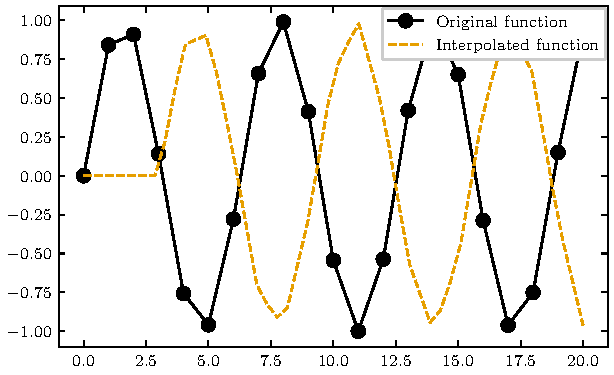
\includegraphics{"images/linear_interpolation_example.pdf"}
	\end{center}
	
	Cubic spline interpolation model of function sin(x) with $N=4$:
	\begin{equation}
		\beta^3(x) = 
		\begin{cases}
			2/3 - |x|^2 + |x|^3/2, & 0 \leq|x| < 1  \\
			(2-|x|)^3/6,           & 1 \leq |x| < 2 \\
			0,                     & 2 \leq |x|     
		\end{cases}
	\end{equation} \cite{main_article}
	
	\begin{center}
		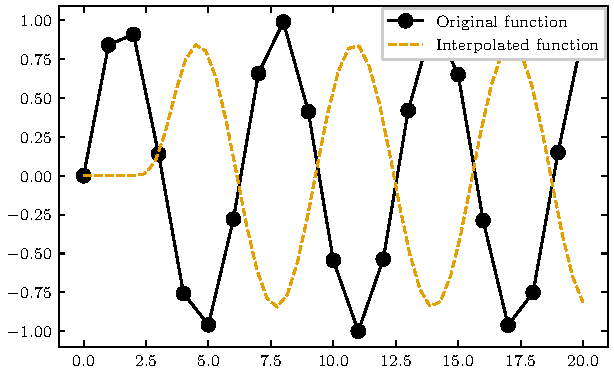
\includegraphics{"images/cubic_interpolation_example.pdf"}
	\end{center}
	
	Standard 2-D interpolation formula for computing the value of the image at location $(x,y)$
	\begin{equation}
		s(x,y) = \sum_{k = k_0}^{k_0+L-1}\sum_{l=l_0}^{l_0+L-1} c(k,l)\varphi(x-k)\varphi(y-l)
	\end{equation}
	
	\fi
	

	\section{Methodology}	
		In this project we will use the same method to rotate an image as in the original paper \cite{main_article} except we will be creating our own convolution kernel in the frequency domain by using a cosine function as base. Defining the function in the Fourier space allows us to fine tune the filter to have a better control over the smoothing effect that will occur when we shift by fractional amounts. Since the kernel will be small we will also just use a normal Inverse Fourier Transform instead of a IFFT. \\
		In the article that this project takes inspiration from it is shown that the traditional rotation matrix
	\begin{equation*}
		R(\theta) = 
		\begin{pmatrix}
			cos\theta & -sin\theta\\
			sin\theta & cos\theta
		\end{pmatrix}
	\end{equation*} 
	can be factorized as three matrices each of which represents a shearing of the image in a cardinal direction.
	\begin{equation*}
		R(\theta) = 
		\begin{pmatrix}
			cos\theta & -sin\theta\\
			sin\theta & cos\theta
		\end{pmatrix}
		=
		\begin{pmatrix}
			1 & -tan\theta/2\\
			0 & 1
		\end{pmatrix}
		\cdot
		\begin{pmatrix}
			1 & 0\\
			sin\theta & 1
		\end{pmatrix}
		\cdot
		\begin{pmatrix}
			1 & -tan\theta/2\\
			0 & 1
		\end{pmatrix}
	\end{equation*} 
	
	The first matrix shears the image in the $x$ direction by $\Delta_x = -y\cdot tan(\theta/2)$, the second matrix shears the image in the $y$ direction by $\Delta_y = x \cdot sin(\theta)$ and the last matrix shears the image again in the $x$ direction by $\Delta_x$.
	In our case we can represent the image as a one dimensional array ordered row-wise and as such can be thought of as a one dimensional signal. This allows us to shift the array using simple memcpy operations and fractional shifts of the signal by the convolution with a small kernel.
	
	\subsection{Fourier domain}
		
	\subsection{Frequencies of a signal}
	\begin{equation}
		freq_{n} = \lfloor \frac{n}{2} \rfloor + 1 \label{freq_equation}
	\end{equation}
	Visual representation with $n=3$ of the discrete Fourier transform of a function $g(x)$
	
	\begin{equation*}
		G_m = \displaystyle\sum_{k=0}^{N-1}g(k)e^{-i \frac{2\pi}{N}km}
	\end{equation*}
	
	To shift a signal by a fractional amount it is imperative to use the correct frequency when doing so.
	
	Given that for $n$ samples we have $\lfloor \frac{n}{2} \rfloor + 1$ distinct frequencies
	
	
	\begin{figure}
		\centering
		\include{file}
		\caption{Unit circle with N = 3, }
	\end{figure}
	
	Euler's Formula
	\begin{equation}
		e^{ix} = cos(x)  + i sin(x)
	\end{equation}
	
	Useful property:
	\begin{equation}
		\cos(w)= \frac{1}{2}(e^{iw}+ e^{-iw})
	\end{equation}
	
	
	\subsection{Fourier Transform with Shift Theorem}
	Here we derive the shift theorem for a discrete signal starting from the normal Fourier Transform with $g_k$ being our 1D input array, $N$ the number of samples and $m$ the frequency:
	\begin{equation*}
		G_m = \displaystyle\sum_{k=0}^{N-1}g_k[k]e^{-i \frac{2\pi}{N} km}
	\end{equation*}
	
	Now instead of $g_k[k]$, we want $g_k[k - \delta]$ where $\delta$ is the amount we want to shift.
	So the above equation can be rewritten as:
	\begin{equation*}
		Z_m = \displaystyle\sum_{k=0}^{N-1}g_k[k - \delta]e^{-i \frac{2\pi}{N} km}
	\end{equation*}
	
	\begin{equation*}
		Z_m = \displaystyle\sum_{r = 0 - \delta}^{N-1-\delta}g_k[r]e^{-i \frac{2\pi}{N} km}, r = k - \delta 
	\end{equation*}
	
	Since $r = k - \delta$ then $ k = r + \delta$, and as such:
	
	\begin{equation*}
		Z_m = \displaystyle\sum_{r= -\delta}^{N-1 - \delta}g_k[r]e^{-i \frac{2\pi}{N} (r + \delta)m}
	\end{equation*}
	
	We can then separate the exponential:
	
	\begin{equation*}
		Z_m = \displaystyle\sum_{r= -\delta}^{N-1 - \delta}g_k[r]e^{-i \frac{2\pi}{N} rm}e^{-i \frac{2\pi}{N}  \delta m}
	\end{equation*}
	
	And factor it out of the sum:
	
	\begin{equation*}
		Z_m = e^{-i \frac{2\pi}{N}  \delta m} \displaystyle\sum_{r= -\delta}^{N-1 - \delta}g_k[r]e^{-i \frac{2\pi}{N} rm}
	\end{equation*}
	
	The sum now has exactly the same range as before:
	
	\begin{equation*}
		Z_m = e^{-i \frac{2\pi}{N}  \delta m} \displaystyle\sum_{k=0}^{N-1}g_k[k]e^{-i \frac{2\pi}{N} km}
	\end{equation*}
	
	\begin{equation}
		Z_m = e^{-i \frac{2\pi}{N}  \delta m} G_m = H_m \cdot G_m \label{shift_equation}
	\end{equation}
	
	
	The above equation \ref{shift_equation} works well for any kind of shift that we want to perform on our signal but for any fractional amount we encounter some problems with the use of the correct frequency indexes.
	Here is a graphical example that was found to be useful: With an $N=3$ number of samples of a signal we have exactly $2$ distinct frequencies \ref{freq_equation} but the total frequencies are actually $3$ and they are $[0+i0, \frac{1}{2}+i\frac{\sqrt{3}}{2}, \frac{1}{2}-i\frac{\sqrt{3}}{2}]$. The last two frequencies are one the complex conjugate of the other.
	
	"Explain why".\\
	To solve this we need to take into consideration the negative frequencies and in particular if the number of samples is odd or even.
	Normally we multiply each sample by its corresponding phase, which is based on the frequency number $m$
	but since we need to take into consideration the negative frequencies we can define a function called wavenum that returns the correct frequency index to use in the phase shift:
	\begin{equation*}
		wave\_n(m) = (m + \lfloor N/2 \rfloor ) \bmod N - \lfloor N/2 \rfloor
	\end{equation*}
	
	\begin{figure}[h]
		\centering
		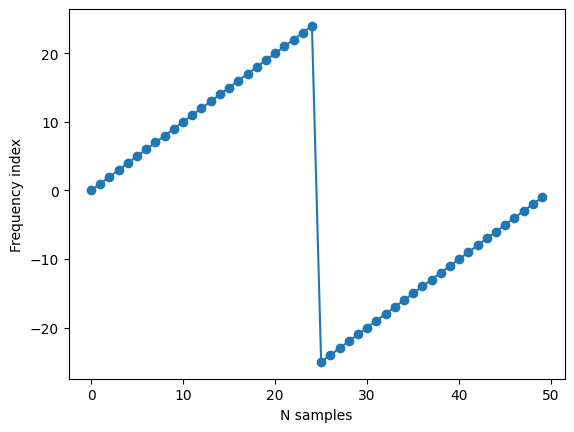
\includegraphics[width=0.5\columnwidth]{images/wavenum_n50.png}
		\caption{Wavenum function with $N=50$}
	\end{figure}
	
	\begin{equation*}
		H_m = e^{-i \frac{2\pi}{N}  \delta \text{wave}\_n(m)}
	\end{equation*}
	
	\begin{equation}\label{phase_shift_equation}
		Z_m = H_{\text{wave}\_n(m)} \cdot G_m
	\end{equation}	
	
	
	
	\subsection{Filter}
	To start of we create the kernel by defining it in the Frequency domain with the use of the Continuous Fourier transform on a sinusoid function.
	\begin{equation}
		F(\omega) = \int_{-M}^{M} \cos(\frac{\pi}{M}t)\mathrm{e}^{-\mathrm{i}\omega t},\mathrm{d}t
	\end{equation}
	This equation allows us to define our CFT in an interval $M$, that we choose based on the fractional amount we want to shift, as to alleviate the oscillations and smoothing that occur with different sizes of M.
	\begin{equation}\label{filter_formula}
		F(\omega) = \frac{2M^2\omega \sin(M\omega)}{M^2\omega^2-\pi^2}
	\end{equation}
	
	Using this function we can build the following filters:
	
	% Filters.
	\begin{figure}[h]
		\centering
		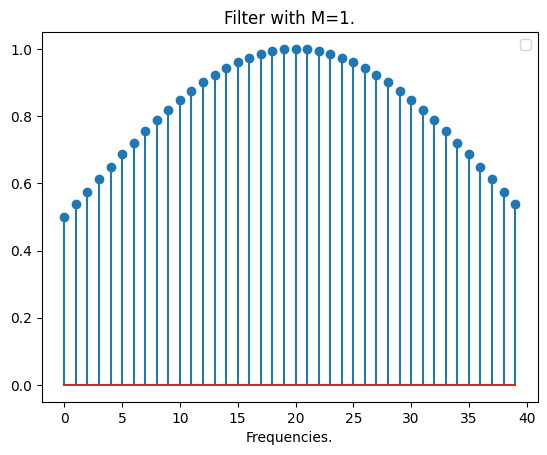
\includegraphics[width=0.4\columnwidth]{images/filter_m_1.png} \hfill		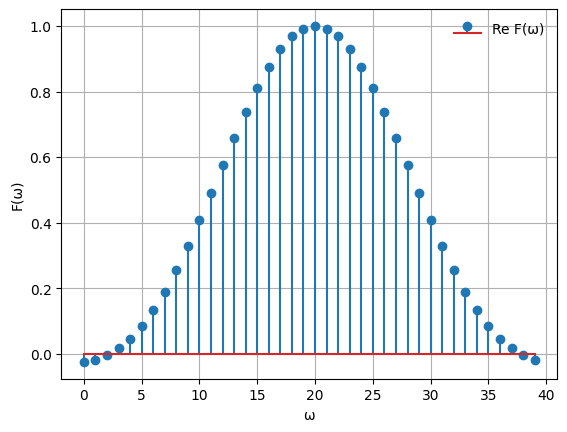
\includegraphics[width=0.4\columnwidth]{images/filter_m_1_5.png} \\
		\parbox{0.4\columnwidth}{\centering Filter with M = 1.} \hfill
		\parbox{0.4\columnwidth}{\centering Filter with M = 2.}
		\centering
		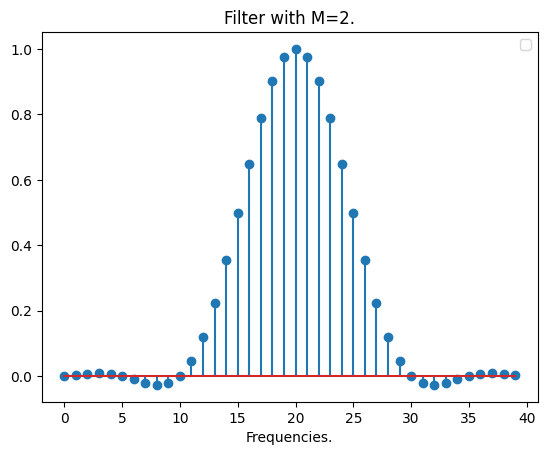
\includegraphics[width=0.4\columnwidth]{images/filter_m_2.png} \hfill		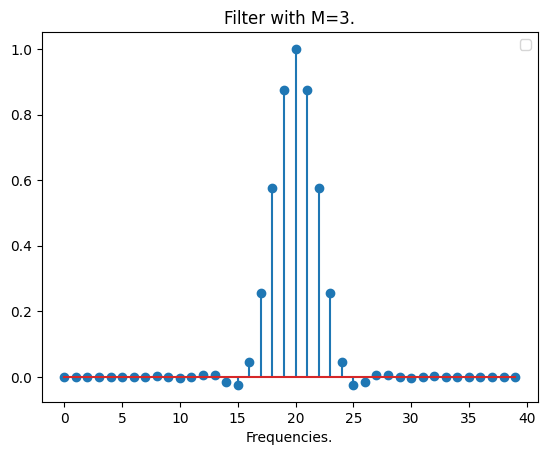
\includegraphics[width=0.4\columnwidth]{images/filter_m_3.png} \\
		\parbox{0.4\columnwidth}{\centering Filter with M = 2.} \hfill
		\parbox{0.4\columnwidth}{\centering Filter with M = 3.}
		\caption{Filter}
		\label{filters}
	\end{figure}
	%
	
	For better accuracy we generally choose our interval M to be small when we have a small fractional shift and big when we have a fractional shift that gets closer to $0.5$. We could write a simplex expression that defines M as:
	\begin{equation*}
		M = 
		\begin{cases}
			1.5 & if 0.1 < x < 0.3\\
			2 & if 0.3 < x < 0.5
		\end{cases}
	\end{equation*}
	
	With some experimenting we found that the filter with $M=3/2$ is a good compromise between smoothing the values and keeping them as accurate as possible. for any fractional shift. 
	
	
	Now that we have our filters we can shift them by the fractional amount in the same way that we defined in equation \ref{shift_equation}. If for example we want to shift our original signal by $10.45$ we will start by creating our filter with $M=\frac{3}{2}$. Then we will apply a shift of $.45$ to the filter:
	
	\iffalse

	
	\begin{figure}[h]
		\centering
		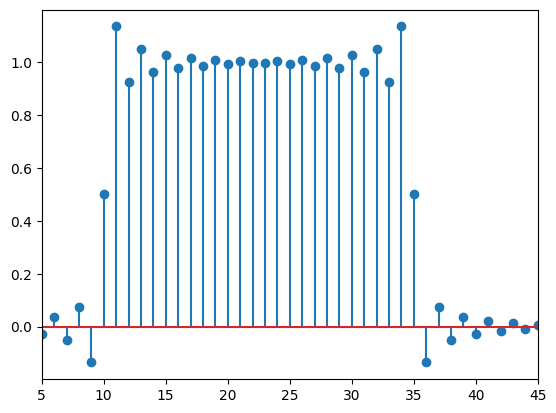
\includegraphics[width=0.5\columnwidth]{images/box_shifted_delta10_1_n50.png}
		\caption{Shifted function by $\delta=10.5$}
	\end{figure}
	
	\subsection{Lanczos Filter and FIR}
	To alleviate the problems that arise when shifting a signal by a fractional amount we can use a filter $L$ that is convoluted with the shifted signal.
	
	\begin{align*}
		L_m &= \frac{\sin(a)}{a},\\
		a &= \frac{2\pi wave\_n(m)}{N}
	\end{align*}
	
	Apply lanczos filter to fractional shift to smooth the result.
	
	\begin{equation*}
		Z_m = L_m \cdot H_m \cdot G_m
	\end{equation*}
	
	\begin{figure}[h]
		\centering
		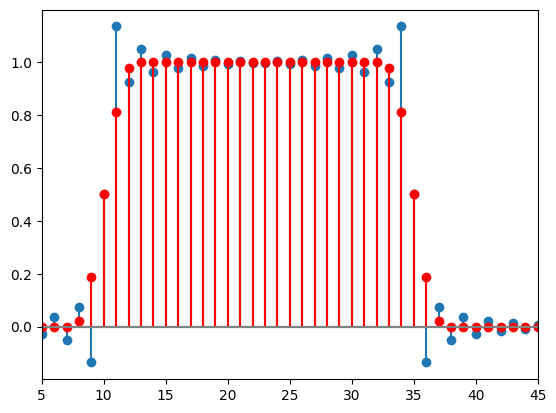
\includegraphics[width=0.5\columnwidth]{images/box_shifted_lanczos_delta10_1_n50.png}
		\caption{Shifted function by $\delta=10.5$ with lanczos filter applied (red), no filter(blue).}
	\end{figure}
	
	\fi
	
	\newpage
	
	\section{Implementation and Project Design}
		The project was mainly done with just a few tools such as: MakeFile, CMake, Jupyter Notebook and some built-in libraries of C and Python like numpy and matplotlib.
		Since the premise of this project is based on the fact that a rotation can be performed with three 1D operations, the bottom-up approach was a no-brainer. We started with the fundamentals of signal processing by exploring the Fourier Transform and Shift Theorem to build our shift kernel. We used Jupyter Notebook extensively to test our method and quickly plot the results, while also documenting everything so that it would be easy to write this report. Since we used the bottom-up approach we were able to re-use parts of the code to test some other aspect of the shift. We started with simple shifts of a 1D signal by an integer value which proved to be quite simple and then we tried to shift the same signal by a fractional amount. This is where some problems arose because some care is needed while shifting each frequency by the correct phase shift.
		
		
	\subsection{Libraries}
		Numpy and Matplotlib were a huge help in plotting the results of our initial tests of the Foruier Transform and of the final results as well. Even for code that was written in C we would then output the binary result to a file and then read that file in python to use matplotlib ton plot the result. There are a few plotting libraries for C but we felt that this was just the faster solution.
		The whole project started out as a CMake and this was chosen mainly because I was already familiar with this tool and was able to quickly setup an environment that would easily build the executables. However towards the end we decided to just use a plain Makefile to keep everything nice and simple.
		
		\subsection{Creating a Filter in the Frequency domain}
		So first off we need to build our kernel. As an example we will create one of size $40$ with $M=2$ since we will be shifting by a fractional amount. To create the kernel then we follow equation \ref{filter_formula}, while also paying attention to evaluating the limit when $\omega=\frac{\pi}{M}$ or $\omega=-\frac{\pi}{M}$. This gives us:
		\begin{figure}[h]
			\centering
			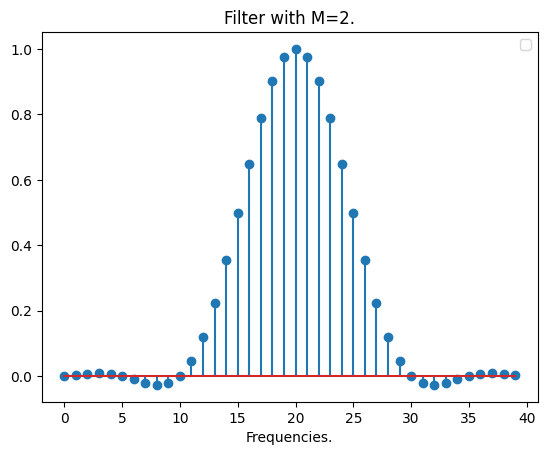
\includegraphics[width=0.4\columnwidth]{images/filter_m_2.png}
			\caption{Filter with $M=2$}
			\label{original_filter}
		\end{figure}
		
		
		
		Now let us say that the fractional amount to shift is $0.25$. To implement this we can use a simple for loop that multiplies each frequency value of the filter by it's corresponding shift \ref{phase_shift_equation}.
		\begin{figure}[h]
			\centering
			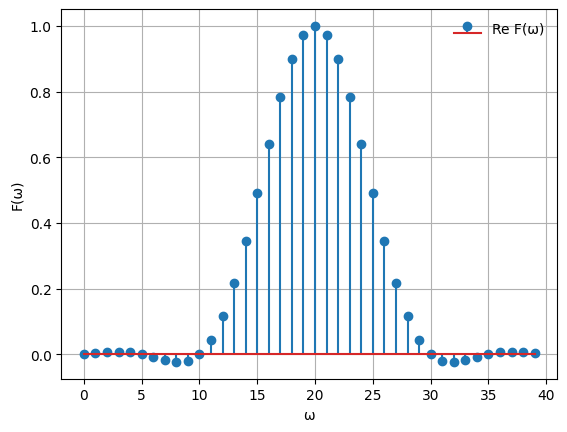
\includegraphics[width=0.4\columnwidth]{images/filter_m_2_25_shift.png}
			\caption{Filter with $M=2$ after shift of $0.25$}
			\label{shifted_filter}
		\end{figure}
		
		 Afterwards we implmented a simple version of the inverse fourier transform, which give us our signal in the time domain. Before returning the result however we need to perform the equivalent of numpy's fftshift function to have the filter values centered. This whole operation can be done in serial and with no real optimization of the code since the kernel size will always be much smaller than the input signal and as such will no be computationally expensive.
		 \begin{figure}[h]
		 	\centering
		 	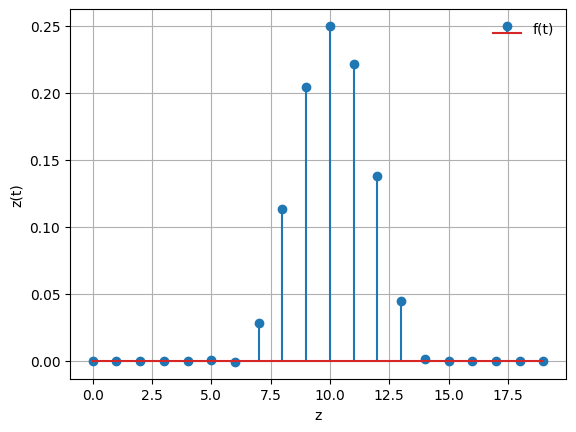
\includegraphics[width=0.4\columnwidth]{images/ifft_filter_m_2_25_shift.png}
		 	\caption{Filter with $M=2$ in spatial domain.}
		 	\label{final_filter}
		 \end{figure}
		 
		 
		
		Here is some pseudo-code that exaplain what is being done to our original filter:
		\begin{algorithm}
			\caption{Filter shift}\label{alg:cap}
		\end{algorithm}
		
		
		\subsection{Convolution Implementation}
		To keep our one dimensional convolution as simple and as efficient as possible we analized it using a Web tool called "Compiler Explorer"\cite{godbolt}. This tool allows us to see which assembly code is being used to perform the convolution operation and choose which implementation should run faster on certain compilers and CPU's.
		
		
		
		\subsection{Integer Shift}
		The end goal has always been to shift by any real value so now we need to handle the integer part of the shift. First of all we need to clarify that if the shift does not have a fractional part then we skip all of the filter creation and convolution and just follow the simple operation that is defined here.
		To shift a signal by an integer amount we will be using the C function \textsl{memcpy} to copy the values of the original array to a resulting array but at a different position, which is defined by the integer shift.
		
		
		
		\section{Results}
		\subsection{Results with 1D signals.}
		\subsection{Results on 2D signals, i.e images}
		
		
		\section{Conclusion}
		
		\section{Future works}
		
		
	
	
	To implement the one dimensional convolution we tried the optimize the algorithm by using godbolt. We came up with a solution that creates the required convolution function at compile time that will perform better than with standard for loops: Go into detail.
	
	Once the fractional shift of our one dimensional signal is over we can just perform a memory copy for the integer part of the shift.
	
	
	
	
	
	\iffalse	
	Explain 1D,2D,3D transposition.
	Simplification of 2D rotation using 1D translations.
	
	Bottom-up , start with 1d kernel then build 2d kernels starting from 1d.
	

	\section{Implementation}
	\begin{itemize}
		\item Problems while implementing the code
		\item Indexing frequencies...
		\item practical problems...
	\end{itemize}
	
	\section{Result}
	
	
	\begin{itemize}
		\item Rotate image many times like in the paper
		\item look for artefacts
		\item compare with C code gathernoloss.c
		\item quality, quantity
	\end{itemize}
	
	
	\section{Solution}
	\section{Validation}
	\section{Conclusion}
	\begin{itemize}
		\item Summary
		\item limitations
	\end{itemize}
		\fi
	\bibliographystyle{plain}
	\bibliography{references}
	
	
\end{document}